\tikzset{%
    every neuron/.style={
        circle,
        draw,
        minimum size=4pt,
        inner sep=0pt,
        very thin
    },
    neuron/.style={
        fill
    },
}
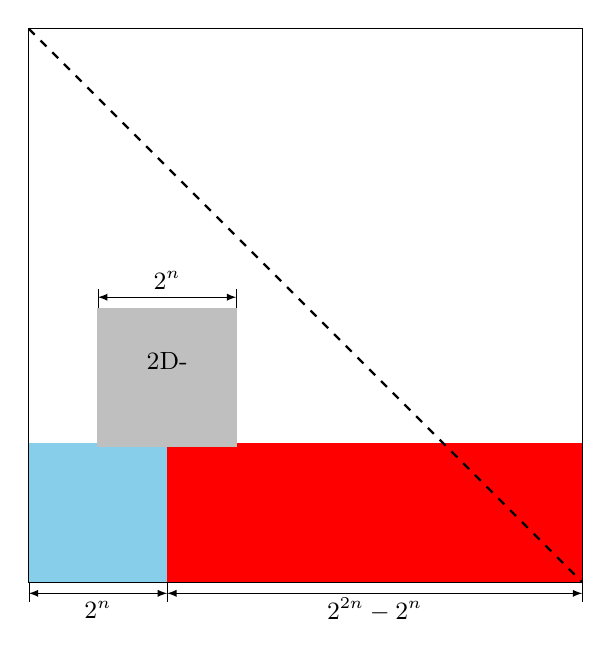
\begin{tikzpicture}[x=0.8cm, y=0.8cm, >=latex, every text node part/.style={align=center}]
    \filldraw [fill=SkyBlue,draw=SkyBlue] (0pt,0pt) rectangle (50pt,50pt);
    \filldraw [fill=Red, draw=Red] (50pt,0pt) rectangle (200pt,50pt);
    \draw [draw=Black] (0pt,0pt) rectangle (200pt,200pt);
    \filldraw [fill=lightgray, draw=lightgray] (25pt, 49pt) rectangle (75pt, 99pt);
    \node [] () at (50pt,74pt) {\small $2$D-\\\footnotesize \Brouwer};
    \path[line width=0.8pt, dashed] (0pt, 200pt) edge (200pt, 0pt);

    \path[line width=0.2pt] (0pt, 0pt) edge (0pt, -7pt);
    \path[line width=0.2pt] (50pt, 0pt) edge (50pt, -7pt);
    \path[<->, line width=0.2pt] (0pt, -4pt) edge (50pt, -4pt);
    \node[] () at (25pt, -10pt) {\small $2^n$};

    % \path[line width=0.2pt] (50pt, 0pt) edge (50pt, -7pt);
    \path[line width=0.2pt] (200pt, 0pt) edge (200pt, -7pt);
    \path[<->, line width=0.2pt] (200pt, -4pt) edge (50pt, -4pt);
    \node[] () at (125pt, -10pt) {\small $2^{2n}-2^n$};

    % \path[line width=0.2pt] (0pt, 0pt) edge (-7pt, 0pt);
    % \path[line width=0.2pt] (0pt, 50pt) edge (-7pt, 50pt);
    % \path[<->, line width=0.2pt] (-4pt, 0pt) edge (-4pt, 50pt);
    % \node[] () at (-10pt, 25pt) {\small $2^n$};

    % % \path[line width=0.2pt] (50pt, 0pt) edge (50pt, -7pt);
    % \path[line width=0.2pt] (0pt, 200pt) edge (-7pt, 200pt);
    % \path[<->, line width=0.2pt] (-4pt, 200pt) edge (-4pt, 50pt);
    % \node[] () at (-10pt, 125pt) {\small $2^{2n}$\\\small $-$\\ \small $2^n$};

    \path[line width=0.2pt] (25pt, 99pt) edge (25pt, 106pt);
    \path[line width=0.2pt] (75pt, 99pt) edge (75pt, 106pt);
    \path[<->, line width=0.2pt] (25pt, 103pt) edge (75pt, 103pt);
    \node[] () at (50pt, 109pt) {\small $2^n$};
\end{tikzpicture}